%!TEX root = ../Main.tex

% ---------------------------------------------------------
\section{Streams and Flows}

A \emph{stream} is an array of elements where the indexing dimension is time. As each element is read from the stream it is available only in that moment, and if the consumer wants to re-use the element at a later time it must save it itself. A \emph{flow} is a bundle of related streams, where each stream carries data from a single partition of a larger data set --- we might create a flow consisting of 8 streams where each one carries data from a 1GB partition of a 8GB data set.

\eject
In our API we manipulate flow endpoints rather than the flows themselves. We use the following data types:

\begin{code}
data Sources i m e 
   = Sources
   { arity :: i
   , pull  :: i -> (e -> m ()) -> m () -> m () }

data Sinks   i m e 
   = Sinks   
   { arity :: i
   , push  :: i -> e -> m ()
   , eject :: i -> m () }
\end{code}

Type @Sources i m e@ classifies flow sources which produce elements of type @e@, using some monad @m@, where the streams in the bundle are indexed by values of type @i@. Likewise @Sinks i m e@ classifies flow sinks which consume elements of type @e@.

In the @Sources@ type, field @arity@ stores the number of individual streams in the bundle. To receive data from a flow producer we use the function in the @pull@ field, passing the index of type @i@ for the desired stream, an \emph{eat} function of type @(e -> m ())@ to consume an element if one is available, and an \emph{eject} function of type @(m ())@ which will be called when no more elements will ever be available for the specified stream. The pull function will then perform an @(m ())@ computation before either calling our eat or eject function, depending on whether data is available from the source.

In the @Sinks type@, field @arity@ stores the number of individual streams as before. To send data to a flow consumer we call the @push@ function, passing the stream index of type @i@, and the element of type @e@. The @push@ function will perform an @(m ())@ computation to consume the provided element. If no more data is available we instead call the @eject@ function, passing the stream index of type @i@, and this function will perform an @(m ())@ computation to shut down the sink --- possibly closing files or disconnecting sockets.

Consuming data from a @Sources@ and producing data to a @Sinks@ is synchronous, meaning that at runtime the computation will block until either an is produced or no more elements are available (when consuming); or an element is consumed or the endpoint is shut down (when producing). In itself the duality between source and sink, push and pull, is folklore, and has previously been used for code generation in array processing languages~\cite{Claessen:ExpressiveArray,Svensson:Defunctionalizing} and XML processing pipelines~\cite{Kay:YouPull}. However, we are not aware of an existing stream processing library based around the simple data types above.

Finally, note that the @eject@ functions used in both the @Sources@ and @Sinks@ type are associated with a single stream only. If our flow consists of 8 streams attached to 8 separate files then ejecting a single stream will close a single file.


% ---------------------------------------------------------
\subsection{Sourcing, Sinking and Draining}
Figure~\ref{f:Draining} gives the definitions of @sourceFs@, @sinkFs@ which create flow sources and sinks based on a list of files, as well as @drainP@ which pulls data from a flow source and pushes it to a sink. 

Given the definition of the @Sources@ and @Sinks@ types, writing @sourceFs@ and @sinkFs@ is straightforward. In @sourceFs@ we first open all the provided files, yielding file handles for each one, and the @pull@ function for each stream source reads data from the corresponding file handle. When we reach the end of a file we eject the correponding stream. In @sinkFs@, the @push@ function for a stream simply writes the provided element to the corredponding file, and the @eject@ function closes it.

The @drainP@ function takes a bundle of stream @Sources@, a bundle of stream @Sinks@, and drains all the data from each source into the corresponding sink. Importantly, @drainP@ forks a separate thread to drain each stream, making the system data parallel. We use intermediate Haskell MVars to communicate between the worker threads and the main threads. After forking all the workers the main threads waits until they are all finished. Now that we have the @drainP@ function, we can copy a partitioned data set from one set of files to another, in parallel:

\begin{code}
 copySetP :: [FilePath] -> [FilePath] -> IO ()
 copySetP srcs dsts
  = do  ss <- sourceFs srcs
        sk <- sinkFs   dsts
        drainP ss sk
\end{code}

In our concrete implementation we also include a @drainS@ (sequential) which evaluates each stream in turn rather than concurrently.

\begin{figure}
\begin{code}
sourceFs :: [FilePath] -> IO (Sources Int IO Char)
sourceFs names 
 = do hs <- mapM (\n -> openFile n ReadMode) names
      let pulls i ieat ieject
          = do let h = hs !! i
               eof <- hIsEOF h
               if eof then hClose   h >> ieject
                      else hGetChar h >>= ieat
      return (Sources (length names) pulls)

sinkFs  :: [FilePath] -> IO (Sinks Int IO Char)
sinkFs names 
 = do hs <- mapM (\n -> openFile n WriteMode) names
      let pushs  i e = hPutChar (hs !! i) e
      let ejects i   = hClose   (hs !! i)
      return (Sinks (length names) pushs ejects)

drainP :: Sources i IO a -> Sinks i IO a -> IO ()
drainP (Sources i1 ipull) (Sinks i2 opush oeject)
 = do mvs <- mapM makeDrainer [0 .. min i1 i2]
      mapM_ readMVar mvs
 where
  makeDrainer i = do
    mv <- newEmptyMVar
    forkFinally (newIORef True >>= drainStream i)
                (\_ -> putMVar mv ())
    return mv
  drainStream i loop =
    let eats v = opush i v
        ejects = oeject i >> writeIORef loop False
    in  while (readIORef loop) (ipull i eats ejects)
\end{code}
% This was the best I could do with the updated drainP function.
% I think the 'while' function is obvious enough to not be defined.

\caption{Sourcing, Sinking and Draining}
\label{f:Draining}
\end{figure}


% ---------------------------------------------------------
\subsection{Stateful Streams, Branching and Linearity}
\label{s:Linearity}
Suppose we wish to copy our set of files while counting the number of characters.
To compute the count we map each character to its individual count --- one --- using @map_o@, described in \S\ref{s:Mapping}.
We sum these with @fold_o (+) 0@, which returns a sink to push the individual counts into and an @IORef@ where the final value will be stored, and takes the arity of the sinks as an argument.

\begin{code}
fold_o :: Ord i => (a -> a -> a) -> a -> i
                -> IO (Sinks i IO a, IORef a)
\end{code}

Trying to drain the source flow into two separate sinks does not work, which is a key part of the design of our system. We might try something like:

\begin{code}
badCopyCount :: [FilePath] -> [FilePath] -> IO Int
badCopyCount srcs dsts
 = do  ss      <- sourceFs srcs
       sk1     <- sinksFs  dsts
       drainP ss sk1
       (sk2,r) <- fold_o (+) 0 (arity ss)
       drainP ss (map_o (const 1) sk2)
       readIORef r
\end{code}

This cannot work. The @Sinks@ endpoint created by @sourceFs@ is a stateful object -- it represents the current position in each of the source files being read. After we have applied the first @drainP@, we have already finished reading through all the source files, so draining the associated flow again does not yield more data. 

Each of the drain computations is performed in the IO monad, which enforces an explicit notion of sequence. The second drain happens after the first one. To copy and count the source data using two separate drain stages we would need to either rewind the file handles attached to the sources, or buffer the data read from the files in memory. Both options are bad. An object of type @Sources@ is an abstract producer of data, and in general it may not be possible to rewind it to a previous state --- suppose it was connected to a stream of sensor readings. On the other hand, buffering all the data read from the flow source so that we can write the output files and then count does not work when the source contains more data than will fit in memory. Instead, we introduce an explicit combinator which branches our flow:

\begin{code}
dup_ooo :: (Ord i, Monad m)
       => Sinks i m a -> Sinks i m a -> Sinks i m a
dup_ooo (Sinks n1 push1 eject1) 
        (Sinks n2 push2 eject2)
 = let pushs  i x = push1 i x >> push2 i x
       ejects i   = eject1 i  >> eject2 i
   in  Sinks (min n1 n2) pushs ejects
\end{code}

The @dup_ooo@ combinator takes two separate sinks and creates a new one. When we push an element to the new sink it will push that element to the two original sinks. Likewise, when we eject the new sink it will eject the two original sinks. We can use this new combinator to write a working @copyMultiple@ function:

\begin{code}
copyCountP :: [FilePath] -> [FilePath] -> IO Int
copyCountP srcs dsts
 = do  ss      <- sourceFs srcs
       sk1     <- sinkFs   dsts
       (sk2,r) <- fold_o (+) 0 (arity ss)
       drainP ss (dup_oo sk1 (map_o (const 1) sk2))
       readIORef r
\end{code}

This new @copyMultiple@ function runs in constant space, which is the behaviour we wanted. Importantly, in the new function definition there is only a single occurrence of each of the variables bound to sources and sinks: @ss@, @sk1@, @sk2@. Each source and sink is used linearly. Our program expresses a data flow graph, where the functions @sourceFs@, @sinkFs@, @fold_o@, @map_o@ and @dup_ooo@ create nodes, and the use-def relation of variables defines the edges.


% ---------------------------------------------------------
\subsection{Polarity and buffering}
In the previous section, @dup_ooo@ branches a flow by taking two existing sinks and produces a new one. The @_ooo@ suffix stands for ``output, output, output'', referring to the three sinks. It turns out that the converse @dup_iii@ combinator is not implementable without requiring unbounded buffering. Such a combinator would have the following type:
\begin{code}
 dup_iii :: (Ord i, Monad m)
         =>  Sources i m a 
         -> (Sources i m a, Source i m a)
\end{code}

Consider how this would work. The @dup_iii@ combinator takes an argument source and produces two result sources. Now suppose we pull data from the left result source. The combinator would need to pull from its argument source to retrieve this data, then when we pull from the right result source we want the same data. The problem is that there is nothing stopping us from pulling the entire stream via the left result source before pulling any elements from the right result source, so @dup_iii@ would need to introduce an unbounded buffer to store all elements in the interim.

Interestingly, although @dup_iii@ cannot work without an unbounded buffer, a hybrid combinator @dup_ioi@ can. This combinator has the following definition:
\begin{code}
dup_ioi :: (Ord i, Monad m)
        => Sources i m a -> Sinks i m a 
        -> Sources i m a
dup_ioi (Sources n1 pull1) (Sinks n2 push2 eject2)
 = let pull3 i eat3 eject3
        = pull1 i eat1 eject1
        where eat1 x = eat3 x >> push2  i x
              eject1 = eject3 >> eject2 i
   in  Sources (min n1 n2) pull3
\end{code}

The @dup_ioi@ combinator takes an argument flow source, an argument flow sink, and returns a result flow source. When we pull data from the result source the combinator pulls from its argument source and then \emph{pushes} the same data to the argument sink. Similarly to @dup_ooo@, we can use @dup_ioi@ to introduce a branch into the data flow graph \emph{without} requiring unbounded buffering of the input flow. This fact was also noticed in the draft paper~\cite{Bernardy:Duality}, though not explained in detail. The same approach works for any number of argument sinks, for example:
\begin{code}
 dup_iooi
  :: (Ord i, Monad m)
  => Sources i m a -> Sinks i m a -> Sinks i m a
  -> Sources i m a
\end{code}

With @dup_iooi@ when we pull from the result source the combinators pulls from its argument source and pushes the same data to its argument sinks. 

Figure~\ref{f:Polarity} the various options for assigning polarities to the argument and result endpoints of a flow duplication combinator. Sources are indicated with a $\bullet$ and sinks with a $\circ$. We use the mnemonic that the filled $\bullet$ can always produce data (being a source) while the empty $\circ$ can always accept data (being a sink). In the figure the greyed out diagrams are for polarity assignments that would require unbounded buffering, while the solid ones require no buffering.

\begin{figure}
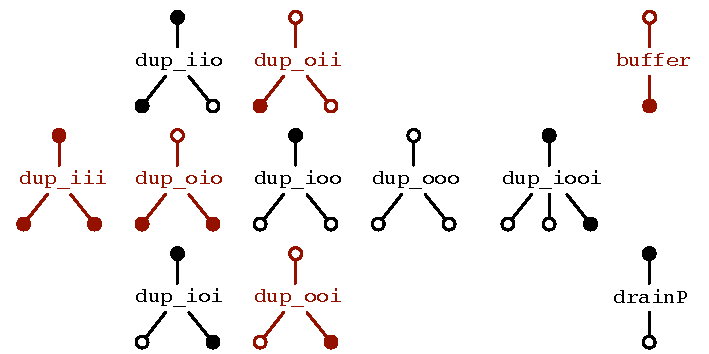
\includegraphics[scale=0.7]{figures/polarity.pdf}

\caption{Possible polarities for the flow duplication combinator}
\label{f:Polarity}
\end{figure}

In the right of Figure~\ref{f:Polarity} we have also included the corresponding polarity diagram for the @drainP@ combinator from Figure~\ref{f:Draining}. The @drainP@ combinator requires no buffering because all data pulled from the source is immediately pushed to the sink. On the other hand, if we invert the polarities of @drainP@ we arrive at the natural assignment for a primitive buffering combinator. A combinator that consumes data via a single argument sink and produces the same data via a result source \emph{must} introduce a buffer as there is no guarantee that new elements are pushed to the sink at the same rate they are pulled from the source. 

Repa library makes it easy to guarantee that data flow programs written with it run in constant space, by only providing combinators with the polarity assignments that do so. This guarantee requires that variables bound to sources and sinks are used linearly, which alas we cannot check with Haskell as it does not support linear types. However, linearity is an easy constraint to understand and check manually, so for now we we leave the job of enforcing it to the client programmer.


% ---------------------------------------------------------
\subsection{Mapping}
\label{s:Mapping}
In Repa Flow, the @map@ operator comes in two forms:
\begin{code}
map_i :: (a -> b) -> Sources i m a -> Sources i m b
map_o :: (b -> a) -> Sinks   i m b -> Sinks   i m a
\end{code}

\begin{figure}
\begin{center}
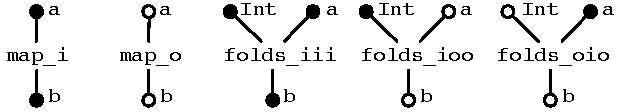
\includegraphics[scale=0.8]{figures/maps.pdf}
\end{center}
\vspace{-0.5em}
\caption{Polarities for \texttt{map} and \texttt{folds}}
\label{f:Map}
\end{figure}

The first form is a source transformer, taking a source of elements of type @a@ and returning a source of elements of type @b@. The second form is a sink transformer, taking a sink of elements of type @b@ and returning a sink of elements of type @a@. The polarity diagram for both forms is given in Figure~\ref{f:Map}. In both cases the elements have type @a@ and the output elements have type @b@. The definition of @map_i@ is as follows. 
\begin{code}
map_i :: (a -> b) -> Sources i m a -> Sources i m b
map_i f (Sources n pullsA)
 = Sources n pullsB
 where  pullsB i eatB ejectB
         = pullsA i eatA ejectA
         where  eatA v = eatB (f v)
                ejectA = ejectB
\end{code}

% We have written this definition using separate let-bindings for each intermediate function, rather than with a single inline lambda abstraction for two reasons:
% \begin{enumerate}
% \item When writing larger functions using contination passing style we begin to feel worringly inside-out. Using intermediate bindings allows us to name each function with the type it expects, which makes the code easier to follow.
% \item It allows us to attach INLINE pragmas to each bound name. This is a critical part of our fusion system, which we will discuss further in \S\ref{s:Chunked}.
% \end{enumerate}

Note that both @map_i@ and @map_o@ are simply flow transformers, and are neither inherently parallel or sequential. Repa Flow supports data parallelism, but parallelism is introduced by the singular @drainP@ function. No other combinator library need be concerned with it. This aspect is similar to the delayed arrays of our original Repa library \cite{Lippmeier:Guiding}, except that parallelism is introduced on a per-stream level rather than a per-element level.


% ---------------------------------------------------------
\subsection{Folding}
Figure~\ref{f:Map} also includes polarity diagrams for three forms of segmented fold. The first one, @folds_iii@ has the following type:
\begin{code}
folds_iii :: (Ord i, Monad m) => (b -> a -> b) -> b
          -> Sources i m Int  -> Sources i m a 
          -> Sources i m b
\end{code}

The @folds_iii@ combinator takes a flow of segment lengths, a flow of elements, and uses the provided combining function and neutral value to fold segments from each stream in the flow. For example, writing flows of streams of elements using nested list syntax we have:
\begin{code}
folds_iii (+) 0 
   [ [3 2 1] [2 2] [4] ] 
   [ [1 2 3 1 1 5] [3 3 4 4] [4 3 2 1] ]
 = [ [6 2 5] [6 8] [10] ]
\end{code}

For the first stream the segment lengths are @[3 2 1]@ and the elements are @[1 2 3 1 1 5]@, we sum up the first three elements, then the next two, then the next one, yielding @[6 2 5]@ for that stream. When @drainP@ from Figure~\ref{f:Draining} is applied to the result source, each of the individual streams in the flow is folded in parallel. We include the definition of @folds_iii@ and the types and definition of the other versions in the appendix.

With @folds_iii@ we assume that both the segment lengths and elements are available as sources. When this is true, evaluation of @folds_iii@ requires no buffering. When we pull a fold result from the result source, the combinator can pull the segment length from its argument source, then the corresponding elements from the element source, folding them in the process. 

As per Figure~\ref{f:Map} it is possible to assign polarities to @folds@ in two other ways that allow the combinator to execute without buffering. 

With @folds_ioo@ we push elements to the element sink (on the right). As needed, the combinator pulls segment lengths from the segment length source (on the left), which instruct it how many of the consecutive elements to fold. As each segment is completed it pushes the result to the result sink (on the bottom).

With @folds_oio@ we push segment lengths to the segment length sink (on the left). As needed, the combinator pulls the corresponding number of elements from the element source (on the right) and folds them. As each segment is completed it pushes the result to the result sink (on the bottom). 

One might wonder if @folds_iii@, @folds_ioo@ and @folds_oio@ are the only versions that can execute without buffering. There are a total of 8 ways of assigning polarities to a 3-leg process such as @folds@. Case analysis reveals that there is one special version:
\vspace{-1ex}
\begin{center}
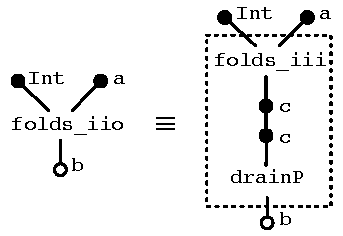
\includegraphics[scale=0.8]{figures/folds-drain.pdf}
\end{center}

\vspace{-1ex}
The @folds_iio@ version can execute without buffering because all the segment lengths and elements in the flow are available as sources, and the result of folding each segment can be pushed directly to the result sink. However, this version is not primitive as it can be expressed as the composition of @folds_iii@ and @drainP@ as shown above. We refer to a combinator version that can be expressed in terms of a composition with @drainP@ as an \emph{active version} because its form implies computation rather than being an \emph{inactive} transformation on sources on sinks. Note that @dup_ioo@ from Figure~\ref{f:Polarity} is also active.

In our concrete library we provide only the combinator versions that execute without buffering, and the only active combinators are @drainS@ and @drainP@. This restriction ensures that it is easy for the client programmer to reason about when computation happens, as well as ensuring that the programs execute in constant space.


% ---------------------------------------------------------
\subsection{Stream projection, funneling, and fattening}
So far the combinators we have discussed have all performed the same operation on each stream of a flow. There are four basic combinators that allow us to convert a flows consisting of several streams into a \emph{singleton} flow, containing only one stream. The endpoints for singleton flows have the index type set to @()@ which indicates there is only one stream in the flow.
\begin{code}
project_i :: i -> Sources i m a -> Sources () m a
project_o :: i -> Sinks   i m a -> Sinks   () m a

funnel_i  :: Sources i IO a -> IO (Sources () IO a)
funnel_o  :: Sinks  () IO a -> IO (Sinks   i  IO a)
\end{code}

The @project@ combinators take a stream index, an endpoint for a flow of several streams, and return a singleton flow containing only data for the specified stream. The @project_i@ combinator takes a source of a flow of several streams, and returns a flow source that selects only the specified stream. The @project_o@ combinator takes a sink for a flow of several streams and returns a sink that discards data for all streams expect the specified stream.

The @funnel@ combinators take an endpoint for a flow of several streams, and return a singleton flow containing data for \emph{all} streams in the argument flow. These combinators expose a duality in the inversion of control associated with such a stream combinator library. 

With @funnel_i@ the order in which the argument streams are processed is under the control of the \emph{combinator} and is \emph{deterministic} when viewed by the consumer of the result source. In our implementation the default order is to present the data from each of the argument streams from the lowest index to highest. Other orders are possible, such as a round-robin process that produces a single element from each non-empty stream in turn. 

In contrast, with @funnel_o@ the order in which argument streams are processed controlled by the \emph{context} and is \emph{non-deterministic} when viewed by the consumer attached to the argument sink. Now, recall that in the implementation of @drainP@ from Figure~\ref{f:Draining} we forked a thread to evaluate each source stream. As each of these threads pushes to its corresponding sink concurrently, if these sinks are then funneled then the order in which elements appear in the output may vary from run to run. As the sink may be attached to a shared resource such as a file, this is also the place in the library where we must introduce locks to manage contention, which is the reason the creation of the result sink must be in the @IO@ monad. Other combinators such as @map@ and @folds@ are lock free, as although they are applied to flow endpoints that conceptually process several streams at once, at runtime there is no communication between threads that evaluate each of these streams.

The fact that @funnel_o@ is more complex to implement than @funnel_i@ stems from the ``central dogma'' of data flow programming: information flows from inputs to outputs, and when information arrives all at once it's harder to deal with. It also suggests a natural program transformation, which we call \emph{drain fattening}:
\begin{alltt}
        (funnel_i s >>= \(\lambda\)s'. drainP s' k)
     => (funnel_o k >>= \(\lambda\)k'. drainP s  k')
\end{alltt}

Which is better expressed as a picture:
\begin{center}
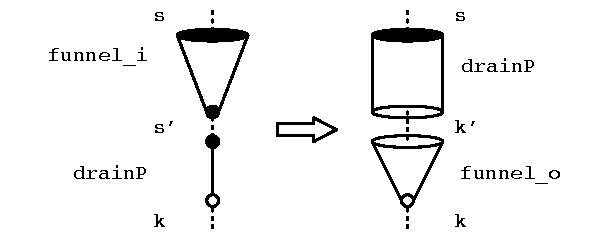
\includegraphics[scale=0.8]{figures/drain-fatten.pdf}
\end{center}

This is valid provided the consumer of the final result source @k@ performs a commutative reduction, or is otherwise insensitive to the order in which elements arrive. By exchanging the order of the @drainP@ and @funnel@ we allow parallel evaluation of multiple streams in the flow, at the expense of introducing non-determinism in the order in which elements are pushed to the sink.

In future work it would be interesting to add a phantom type parameter to our @Sinks@ data type to represent the fact that a particular sink is insensitive to the order in which elements arrive. This would enable us to fatten our drains automatically, but for now the transformation must be performed by hand.

Although fattening can only be applied when a @funnel_i@ is syntactically close to a @drainP@, the fact that our combinators come in a variety of polarized versions allows us to pull many of them through a @drainP@ to bring their arguments closer, for example:
\begin{alltt}
  drainP (map_i f s) k  =  drainP s (map_o f k)
\end{alltt}


\eject

